\documentclass[dvipdfmx]{jsarticle}
\usepackage[dvipdfmx]{graphicx}
\begin{document}


\section*{2.4 レイトレーシング(光線追跡)}
一般的な都市部や屋内環境では,固定された送信源から送信された無線信号は,環境中の複数の物体に遭遇し,その物体は,図2.3に示すように送信信号の反射,回折,散乱コピーを生成する.
マルチパス信号成分と呼ばれる,これらの送信信号の追加のコピーは,受信機において,LOS信号経路と比較して,電力の減衰,時間の遅延,位相や周波数のずれが発生し得る.
受信機では,マルチパス信号と送信信号は合計されるが,送信信号に対する受信信号の歪みがしばしば発生する.

\begin{figure}[htbp]
\begin{center}
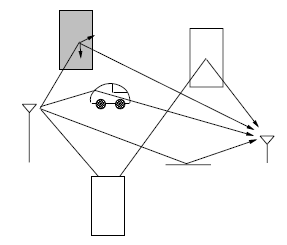
\includegraphics[]{spring_lec/wc_ray.png}
\end{center}
\caption{物体に遭遇し,反射,回折,散乱した波の様子}
\end{figure}

レイトレーシングでは,位置と誘電特性が既知の有限個の反射板を想定している.そして,マルチパス伝搬の詳細は,適切な境界条件とともにマクスウェル方程式を使用して解くことができる.しかし,この解法は計算量が多いため,一般的なモデリングツールとしては実用的ではない.
レイトレーシング技術は,波面を単純な粒子として表現することで,電磁波の伝搬を近似的に表現するものである.したがって,波面の反射,回折,散乱の効果は,Maxwellのより複雑な波動方程式の代わりに,単純な幾何学方程式を使って近似される.レイトレーシング近似の誤差は,受信機が最も近い散乱体から何波長も離れており,すべての散乱体が波長に対して大きく,かつかなり滑らかな場合に最も小さくなる.レイトレーシング法を経験的データと比較すると,農村部\cite{ten},送信機と受信機の両方が地面に近い街路沿い\cite{eight}\cite{seven}\cite{ten},または回折係数を適切に調整した室内環境\cite{nine}で,受信信号電力を正確にモデル化できることが示されている.マルチパスの遅延広がりなど,受信電力変動以外の伝搬効果は,レイトレーシング技術では必ずしもうまく捉えられない\cite{eleven}.

送信機,受信機,反射板がすべて動かない場合,複数の受信信号経路の影響と,LOS経路に対するそれらの遅延は固定される.しかし,送信機や受信機が移動している場合,複数のパスの特性は時間によって変化する.反射板の数,位置,特性が時間的に既知である場合,これらの時間変化は決定論的である.そうでない場合は,統計的モデルを使用しなければならない.
同様に,反射板の数が非常に多い場合や,反射板の表面が滑らかでない場合も,受信信号の特性を把握するために統計的な近似値を使用する必要がある.伝搬効果に関する統計的なフェージングモデルについては,第3章で説明する.光線追跡と統計的フェーディングを組み合わせたハイブリッドモデルも文献\cite{thirteen}\cite{fourteen}で見ることができるが,ここでは説明しない.

最も一般的なレイトレーシング・モデルは,減衰,回折,および散乱されたすべてのマルチパス成分を含む.
このモデルは,送信機と受信機を取り囲む物体の幾何学的特性と誘電体特性をすべて使用する.
ルーセント社のワイヤレスシステムエンジニアリングソフトウェア(WiSE),ワイヤレスバレー社のSitePlannerR,マルコーニ社のPlanetR EVなどのレイトレーシングに基づくコンピュータプログラムは,屋内外の環境でのシステム計画に広く使用されている.これらのプログラムでは,コンピュータグラフィックスを航空写真(屋外チャンネル)または建築図面(屋内チャンネル)と組み合わせて,環境の3D幾何学的な画像を得ることができる\cite{one}.

以下のセクションでは,複雑さを増すいくつかのレイトレーシング・モデルについて説明する.まず,LOS経路に干渉する地上反射の結果生じる信号変動を予測する単純な2光線モデルから始める.このモデルは,地方の道路や高速道路など,反射物が少ない孤立した場所での信号伝搬を特徴付けるものである.屋内環境では一般的に良いモデルとは言えない.次に,直線的な道路や廊下に沿って伝搬する信号の変動を予測する10線反射モデルを紹介する.最後に,あらゆる伝搬環境における信号の伝搬を予測する一般的なモデルについて説明する.2線モデルはアンテナ高さの情報のみを必要とするが,10線モデルはアンテナ高さと道路/廊下の幅の情報を必要とし,一般モデルはこれらのパラメータに加えて,環境中の反射器,回折器,散乱器の形状や誘電特性に関する詳細な情報を必要とする.

\renewcommand{\refname}{文献一覧}
\begin{thebibliography}{99}
\bibitem{ten}T. Kurner, D.J. Cichon, andW.Wiesbeck, “Concepts and results for 3D digital terrain-basedwave propagation models: an overview,” IEEE J. Select. Areas Commun. pp. 1002–1012, Sept. 1993.
\bibitem{eight}N. Amitay, “Modeling and computer simulation of wave propagation in lineal line-of-sight microcells,” IEEE
Trans. Vehic. Technol., Vol VT-41, No. 4, pp. 337–342, Nov. 1992.
\bibitem{seven}J.W. McKown and R.L. Hamilton, Jr., “Ray tracing as a design tool for radio networks,” IEEE Network , Vol.
5, No. 6, pp. 27–30, Nov. 1991.
\bibitem{nine}K. A. Remley, H. R. Anderson, and A. Weisshar, “Improving the accuracy of ray-tracing techniques for
indoor propagation modeling,” IEEE Trans. Vehic. Technol., pp. 2350–2358, Nov. 2000.
\bibitem{eleven}H.-J. Li, C.-C. Chen, T.-Y. Liu, and H.-C. Lin, “Applicability of ray-tracing techniques for prediction of
outdoor channel characteristics,” IEEE Trans. Vehic. Technol., pp. 2336–2349, Nov. 2000.
\bibitem{thirteen}A. Domazetovic, L.J. Greenstein, N. Mandayan, and I. Seskar, “A new modeling approach for wireless channels
with predictable path geometries,” Proc. IEEE Vehic. Technol. Conf, Sept. 2002.
\bibitem{fourteen}J.H. Tarng, W.-S. Liu, Y.-F. Huang, and J.-M. Huang, “A novel and efficient hybrid model of radio multipathfading
channels in indoor environments,” IEEE Trans. Ant. Prop., Vol. 51, pp. 585 - 594, March 2003.
\bibitem{one}T.S. Rappaport, Wireless Communications - Principles and Practice, 2nd Edition, Prentice Hall, 2001.
\end{thebibliography}
\end{document}